The following description is derived from the work of Rahm and Do \cite{Rahm2000DataApproaches}.
In its essence data cleaning aims to improve the overall quality of data.
This goal is achieved by removing errors, noise, duplicates, inconsistencies and misspellings from datasets.
Especially when multiple data sources are being integrated into a single set the need for data cleaning becomes apparent.
Different sources often feature varying representations of the same data.

As this visualization pulls in data from heterogeneous sources (Section \ref{sec:source-integration}) common data cleaning techniques are applied for consolidation.
There are four areas of concern: (1) Linking the scientific Latin name, (2) filtering non-animal entries, (3) enriching abbreviations with labels and (4) establishing a common relational schema.
The following sections elaborate on these areas in detail.

\subsubsection{Name Linking}
The \textit{Taxon} field of the CITES Wildlife dataset contains the scientific name of an animal in Latin.
While a direct connection to the IUCN API can be established using the Latin taxonomic name it is not suitable for data analysis (without a background in Biology) nor for usage in the final visualization.
Therefore, taxonomic names should be mapped to their English common counterpart.
Querying the IUCN API allows the retrieval of common names in one or more languages.

\begin{lstlisting}[caption={Retrieving common names of the red panda from the IUCN API}, label={lst:iucn-common-names}, language=json]
GET /species/common_names/ailurus%20fulgens
{
  "name": "Ailurus fulgens",
  "result": [
    {
      "taxonname": "Red Panda",
      "primary": true,
      "language": "eng"
    },
    ...
  ]
}
\end{lstlisting}

Collecting a unique set of taxonomic names provides the basis to iteratively query the IUCN API for common names. Listing \ref{lst:iucn-common-names} shows an example query for the red panda using a simple HTTP GET request.

\subsubsection{Non-animal Filter}
This visualization project intentionally focuses on animal wildlife only.
However, the CITES Wildlife database contains both animals and vegetation.
Each non-animal entry should therefore be filtered from the dataset.
There is no binary column indicating to which group an entry belongs.
Instead, the \textit{Term} field describes which type is being imported or exported.
Reducing the \textit{Term} column to its unique values yields 83 distinct types.
These types can manually be flagged when they signify non-animal entries e.g. seeds, dried plants, roots, bark, logs, fruit or leaves.

\subsubsection{Abbreviation Enrichment}
The CITES Wildlife database features five columns containing abbreviations: (1) \textit{Importer}, (2) \textit{Exporter}, (3) \textit{Origin}, (4) \textit{Purpose} and (5) \textit{Source}.
Cutting down the length of repetitive values helps to reduce file size and retains readability in editors.
In order to display these values in a visualization full labels should be used.
This provides an accurate description which does not rely on additional background knowledge.

\textit{Importer}, \textit{Exporter} and \textit{Origin} all contain two-letter country codes in the ISO 3166 alpha-2\footnote{\url{https://www.iso.org/iso-3166-country-codes.html}, accessed: 28-02-2018} format.
\textit{Purpose} and \textit{Source} are specific one-letter codes which can be resolved using the CITES trade guidelines documentation\footnote{\url{https://trade.cites.org/cites_trade_guidelines/en-CITES_Trade_Database_Guide.pdf}, accessed: 28-02-2018}.


\subsubsection{Relational Schema} 
\textcolor{white}{filler}

\begin{figure} [h] 
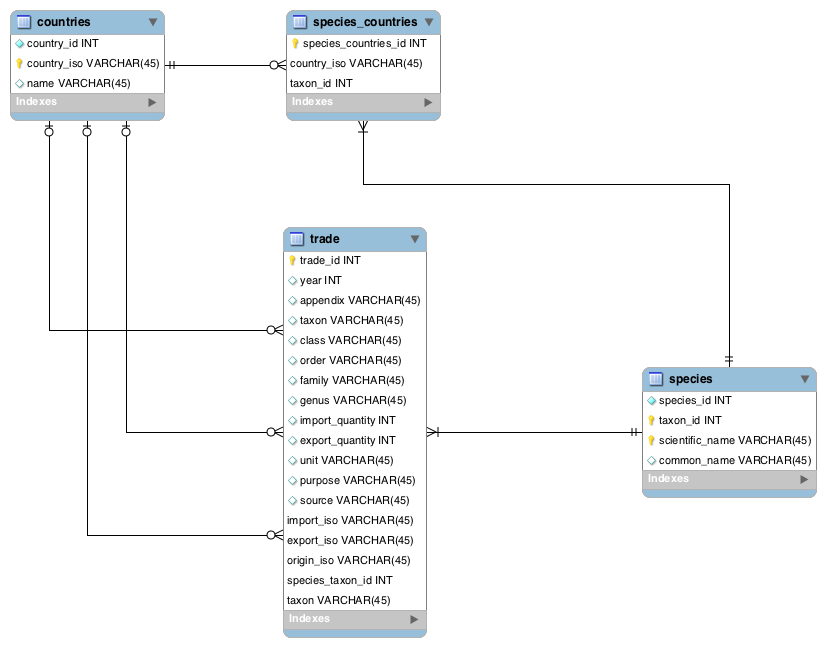
\includegraphics[width=12cm]{images/relation_schema.png}
\caption{Relational Schema}
\label{Relation Schema}
\end{figure}
